\newpage
\section{结构形成理论}
宇宙学原理认为宇宙在足够大的尺度上是均匀, 各向同性的. 实际上在小尺度, 甚至较大尺度上, 宇宙是不均匀的, 并且这种不均匀在目前宇宙中更加明显. 

\begin{align*}
    \delta=\frac{\rho(x)-\bar{\rho}}{\bar{\rho}}
\end{align*}
密度的涨落的扰动导致引力不平衡破坏了稳定性. 

\subsection{流体力学}
均匀宇宙可以看成是一个流体. 流体力学基本方程:
\begin{enumerate}
    \item 连续性方程: 质量守恒, 流出与流入相同
    \begin{align}
        \frac{\partial \rho}{\partial t}+\nabla \cdot (\rho v)=0 \label{EE1}
    \end{align} 
    \item 运动学方程(欧拉方程)
    \begin{align}
        \frac{\partial v}{\partial t}+(v\cdot \nabla)v=-\frac{\nabla p}{\rho}-\nabla \Phi \label{EE2}
    \end{align}
    \item Poisson(泊松方程)
    \begin{align}
        \nabla^2 \Phi=4\pi G\rho \label{EE3}
    \end{align}
\end{enumerate}
上述等式是在欧拉坐标下的描述, 即给定时间, 给定位置处流体的密度、速度的变化情况. 另一种有效的描述是拉格朗日坐标, 即考察某一固定流体元本身的密度, 速度等变化, 在此情况下, 流体性质(密度, 速度, 温度等)只是时间的函数, 其导数一般写为$\frac{d}{dt}$. 

拉格朗日坐标描述与欧拉坐标描述下偏导之间的关系为
\begin{align*}
    \frac{d}{dt}=\frac{\partial }{\partial t}+(v\cdot\nabla)
\end{align*}

考察一个均匀、各向同性宇宙的平衡情况. 对于连续性方程, 由于密度$\rho$与位置$r$无关, 只是时间的函数, 可得
\begin{align*}
    \frac{\partial \rho}{\partial t}+\rho \Delta\cdot v+v \Delta \cdot \rho=\frac{\partial \rho}{\partial t}+\rho\Delta\cdot v=0
\end{align*}
上式中每项都应该是时间的函数, 因此速度$v$应该满足$v=f(t)r$,  令$f(t)=\frac{\dot{a}(t)}{a(t)}$, 代入上式可得
\begin{align*}
    \frac{\partial \rho}{\partial t}+3\rho\frac{\dot{a}}{a}=0
\end{align*}
可得$\rho\sim a(t)^{-3}$(物质守恒).  由球对称下的泊松方程 \ref{EE3}, 可写为
\begin{align*}
    \frac{1}{r^2}\frac{\partial \left( r^2\frac{\partial \Phi}{\partial t} \right)}{\partial r}=4\pi G\rho(t)
\end{align*}
可得$\Phi=\frac{2\pi G}{3}\rho r^2$, 将其代入欧拉方程, 可得
\begin{align*}
    \frac{\ddot{a}}{a}=-\frac{4\pi G}{3}\rho
\end{align*}
该等式正是Friedmann方程之一. 代入物质守恒方程, 可得$a\sim t^{2/3}$. 

可以看到, 完全可以从牛顿定律出发, 得到哈勃定律, 以及宇宙正在膨胀(而且必须膨胀)的解, 其尺度因子与前述求解Friedmann方程完全一样. 

因此, 一个均匀各向同性的宇宙不可能是静止的. 基于宇宙学原理, 任何观测者都会看到一个运动的流体, 因此必然推导出空间的膨胀. 

\subsection{金斯不稳定性}
\subsubsection{静止宇宙下的扰动方程}
假设在平衡态时, 密度$\rho_0$, 速度$v_0$, 满足流体方程
\begin{align*}
    \frac{\partial \rho_0}{\partial t}+\rho_0 \nabla\cdot v_0+v_0 \nabla \cdot \rho_0&=0\\
    \frac{\partial v_0}{\partial t}+v_0 \nabla \cdot v_0+\frac{\nabla P_0}{\rho_0}+\nabla \Phi_0&=0\\
    \nabla^2 \Phi_0&=4\pi G\rho_0
\end{align*}
对于一个相对平衡态的轻微扰动, 有
\begin{align*}
    \rho&=\rho_0+\delta \rho\\
    v&=v_0+\delta v\\
    P&=P_0+\delta P\\
    \Phi&=\Phi_0+\delta \Phi
\end{align*}
将其代入流体方程, 并略去平衡项和高阶项
\begin{align*}
    \frac{\partial \delta\rho}{\partial t}+\rho_0 \nabla\cdot \delta v+\delta \rho \nabla\cdot v_0+\delta v \nabla \cdot \rho_0+v_0 \nabla \cdot \delta \rho&=0\\
    \frac{\partial \delta v}{\partial t}+v_0 \nabla \cdot \delta v+ \delta v \nabla \cdot v_0+\frac{\nabla  \delta P}{\rho_0}+\nabla  \delta \Phi&=0\\
    \nabla^2  \delta \Phi&=4\pi G \delta\rho
\end{align*}
进一步假设密度$\rho_0$均匀, 只是时间的函数, 其流体平衡时处于静止状态$v_0=0$, 可以得到
\begin{align}
    \frac{\partial^2 \delta}{\partial t^2}-c_s^2 \nabla^2\delta-4\pi G \rho_0 \delta=0 \label{EE4}
\end{align}
这里$\delta=\frac{\delta \rho}{\rho_0}$, $c_s^2=\frac{\partial P}{\partial \rho}$为流体的声速. 

\subsubsection{膨胀宇宙下的扰动方程}
均匀各向同性的宇宙不可能处于静止状态, 其存在一个满足流体方程的平衡态解, $\rho\sim a^{-3}, v=\frac{\dot{a}}{a}r$, 结合宇宙学基本概念可知, 这里密度变化与速度量来自宇宙膨胀. 如果将流体方程坐标从$r\rightarrow x (r=ax)$转换到共动坐标$x$下, 则哈勃膨胀项$(v=Hr)$可以忽略. 

可证明, 在$r=ax$时 $(v=\dot{r}=\dot{a}x+a\dot{x}=\dot{a}x+u)$, 将流体方程从坐标$(r,t)$转换到$(x, t)$下, 需要做如下变化
\begin{align*}
    \nabla_r&\rightarrow \frac{1}{a}\nabla_x\\
    \frac{\partial }{\partial t}&\rightarrow \frac{\partial }{\partial t}-\frac{\dot{a}}{a}x\dot\nabla_x
\end{align*}
令$\rho(x,t)=\overline{\rho(t)}(1+\delta(x,t))$, $a\dot{x}=v$, 可得共动坐标下流体方程
\begin{align*}
    \frac{\partial \delta}{\partial t}+\frac{1}{a}\nabla\cdot[(1+\delta)v]&=0\\
    \frac{\partial v}{\partial t}+\frac{\dot{a}}{a}v+\frac{1}{a}(v\cdot \nabla)v&=-\frac{\nabla\Phi}{a}-\frac{\nabla P}{a\bar{\rho}(1+\delta)}\\
    \nabla^2\Phi&=4\pi Ga^2\bar{\rho} \delta\\
    \Phi&=\phi+\frac{a\ddot{a}x^2}{2}
\end{align*}
略去高阶项后可以得到
\begin{align}
    \frac{\partial^2 \delta}{\partial t^2}+2\frac{\dot{a}}{a}\frac{\partial \delta}{\partial t}=4\pi G \bar{\rho}\delta+\frac{c_s^2}{a^2}\nabla^2 \delta \label{EE5}
\end{align}
(共动坐标下的宇宙扰动方程)可以看到, 相比 \ref{EE4}, 膨胀宇宙下扰动方程只多出一个膨胀项, 当$\dot{a}=0$是, 与 \ref{EE4} 等价. 
在密度扰动较小的线性情况下, 实空间的扰动可以表示为傅里叶空间分量之和, 每个傅里叶模独立演化 (类似于不同频率平面波叠加, $k$相当于频率), $\displaystyle \delta(x,t)=\sum_k\delta_k(t)e^{ik\cdot x}$ 代入扰动方程
\begin{align}
    \frac{d^2\delta_k}{d t^2}+2\frac{\dot{a}}{a}\frac{d\delta_k}{dt}=\left( 4\pi G \bar\rho-\frac{k^2c_s^2}{a^2} \right)\delta_k \label{EE6}
\end{align}
可以在不同宇宙学模型下$(a=a(t))$下得到扰动的演化. 
\paragraph{没有宇宙膨胀 \texorpdfstring{$\dot{a}=0$}.}
此时扰动方程 \ref{EE6} 为:
\begin{align*}
    \frac{d^2\delta_k}{d t^2}&=-\omega^2\delta_k\\
    \omega^2&=\left( \frac{k^2 c_s^2}{a^2}-4\pi G\bar{\rho} \right)
\end{align*}
该方程的普适解为$\delta_k(t)=\delta_k(t=0)e^{\pm i\omega t}$, 其定义了一个特征物理尺度, 金斯长度 $\lambda_J\equiv \frac{2\pi a}{k}=c_s\sqrt{\frac{\pi}{G\bar{\rho}}}$, 与原恒星形成类似, 金斯长度定义了一个均匀流体发生坍缩的条件. 
\begin{itemize}\small
    \item 当$\lambda<\lambda_J(k>k_J)$时, $\omega^2>0$, $\omega$为实数, 因此
    \begin{align*}
        \delta_k(t)\sim\delta_k(t=0)e^{\pm iwt}
    \end{align*}
    表示一个声波, 其振幅不发生变化, 在空间以声速传播. 
    \item 当$\lambda>\lambda_J(k<k_J)$时, $\omega^2<0$, $\omega$为虚数, 因此
    \begin{align*}
        \delta_k(t)\sim\delta_k(t=0)e^{\pm iwt}
    \end{align*}
    表示静态波(不传播), 其振幅随时间衰减或增长, 这里只关心增长解. 
\end{itemize}

特殊时刻的金斯波长和金斯质量:
\begin{enumerate}
    \item 再复合以前(before recombination)
    \subitem 再复合之前, 重子处于电离状态, 光子与电子之间频繁发生散射, 因此光子和重子可以视为一种单一流体, 其密度$\rho=\rho_r+\rho_b$, 压强主要由光子主导, 因此声速为 $\displaystyle c_s=\frac{c}{\sqrt{3}}\left[ \frac{3}{4}\frac{\rho_b(z)}{\rho_r(z)}+1 \right]^{-1/2} $, 定义在球半径$\displaystyle\frac{\lambda_J}{2}$的质量为金斯质量$M_J\approx 1.2\times 10^{16}(\Omega_b h^2)^{-2}M_{\odot}$. 因此再复合之前, 只有超过星系团质量的重子物质结构才能增长, 小质量为声波振荡. 
    \item 再复合时期结束时(after recombination)
    \subitem 在recombination结束时, 光子与重子脱藕, 重子气体的声速$\displaystyle c_s=\left( \frac{5kT}{3m_p} \right)^{1/2}$, 该时刻金斯长度(物理尺度)$\displaystyle \lambda_J\sim\frac{0.01}{(1+z_{rec})}(\Omega_b h^2)^{-1/2}Mpc$, 
    \begin{align*}
        M_J\equiv \frac{\pi}{6}\overline{\rho(z_{rec})}\lambda_J^3\sim 1.5\times 10^5(\Omega_b h^2)^{-1/2}M_{\odot}
    \end{align*}
    因此, 复合结束时, 金斯质量的质量与球状星团相当. (大于该质量的结构可以形成)
\end{enumerate}

\paragraph{宇宙膨胀时的解}
宇宙的物质: 光子, 重子物质, 暗物质, 暗能量

\begin{enumerate}
    \item \textbf{物质主导}
    
    \subitem 考虑没有压强项的时候(对于\textbf{暗物质}, 或者扰动尺度远大于金斯长度, 压强项可以忽略),
    扰动方程
    \begin{align*}
        \frac{d^2\delta_k}{d t^2}+2\frac{\dot{a}}{a}\frac{d\delta_k}{dt}= 4\pi G \bar\rho\delta_k 
    \end{align*}
    对物质主导$a\sim t^{2/3}$, 可得$\delta\sim t^{2/3}\sim a$. 结合哈勃常数$H(z)=H(0)*E(z)$, 可对此方程进行数值求解(对z从0积分到给定红移), 其增长解可以写为
    {\small
    \begin{align*}
        \delta_k\propto D(z)&=\frac{g(z)}{(1+z)}\\
        g(z)&\approx \frac{5}{2}\Omega_m(z)/\\
        &\left[ \Omega_m^{4/7}(z)-\Omega_\Lambda(z)+\left( 1+\frac{\Omega_m(z)}{2} \right)\left( 1+\frac{\Omega_\Lambda(z)}{70} \right) \right]
    \end{align*}
    }$\displaystyle \Omega_m(z)=\frac{\Omega_{m,0}(1+z)^3}{E^2(z)},\ \Omega_\Lambda(z)=\frac{\Omega_{\lambda, 0}}{E^2(z)}$. 扰动在没有宇宙学常数情况下增加得更快. (哈勃膨胀减弱了扰动的增长, 因为宇宙学常数导致宇宙膨胀的更快. )
    
    \begin{figure}[!htb]
        \centering
        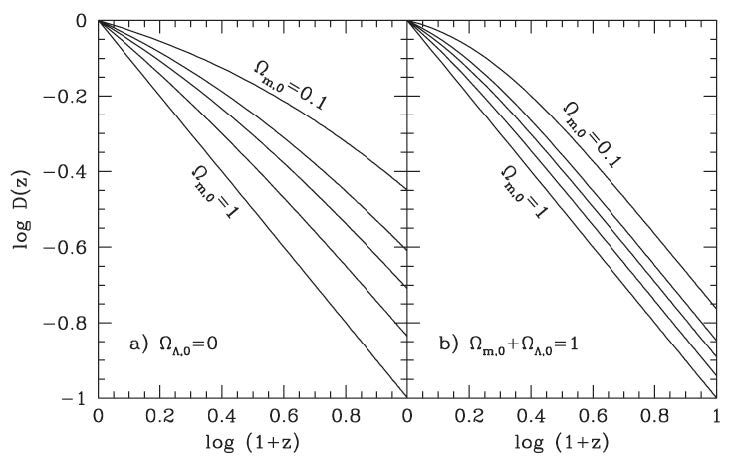
\includegraphics[width=0.42\textwidth]{GA8/几种宇宙学参数下扰动因子随红移的变化}
        \caption{几种宇宙学参数下扰动因子随红移的变化}
    \end{figure}
    
    \subitem 有压强的\textbf{重子物质}扰动, 对于再复合以后, 由暗物质和重子组成的宇宙, 当暗物质密度大于重子密度时, 暗物质的密度演化由前述无压强扰动方程给出. 对于重子, 其引力项由暗物质提供, 但是需要考虑其压强. 扰动方程
    \begin{align*}
        \frac{d^2\delta_k}{d t^2}+2\frac{\dot{a}}{a}\frac{d\delta_k}{dt}+\frac{k^2c_s^2a}{a^3}\delta_b=4\pi G \bar\rho_0\frac{a_0^3}{a^3}\delta_{dm}
    \end{align*}
    存在较普遍的解
    \begin{align*}
        \delta_b(k,t)=\frac{\delta_{dm}(k,t)}{1+k^2/k_J^2}
    \end{align*}
    $\displaystyle k_J^2\equiv \frac{3a^2H^2}{2c_s^2}$. 可以看到
    \begin{itemize}
        \item 当$k\ll k_J, \delta_b=\delta_{dm}$, 即大尺度上, 重子物质扰动与暗物质相当. 
        \item 当$k\gg k_J, \delta_b=\delta_{dm}\frac{k_J^2}{k^2}$, 且由于$a^2H^2\sim t^{-2/3}$, 因此重子的扰动远小于暗物质扰动, 且随着时间增加而衰减. 
    \end{itemize}
    随着宇宙膨胀, 重子温度降低, 其声速降低, 导致$k_J$ 快速变大, 因此, 对任意$k$的扰动, 其很快满足$k\ll k_J$, 因此重子的扰动很快跟上暗物质的扰动. 
    \item \textbf{辐射主导}
    
    \subitem \textbf{光子}的扰动(相对论性流体, 且扰动尺度小于视界): 当宇宙处于辐射主导时期, 必须考虑辐射压对能量密度的贡献, 基本流体方程为
    \begin{align*}
        \frac{\partial \rho}{\partial t}+\nabla\cdot[(\rho+P)v]&=0\\
        \frac{\partial v}{\partial t}+(v\cdot \nabla)v+\frac{\nabla P}{(\rho+P)}+\nabla\Phi&=0\\
        \nabla^2\Phi&=4\pi G(\rho+3P)\\
        &=8\pi G\rho
    \end{align*}
    与前述得到扰动方程类似, 可以得到相对性流体情况下的扰动方程
    \begin{align*}
        \frac{d^2\delta_k}{d t^2}+2\frac{\dot{a}}{a}\frac{d\delta_k}{dt}=\left( \frac{32\pi G \rho}{3}-\frac{k^2c_s^2}{a^2} \right)\delta
    \end{align*}
    唯一差别为引力项中, 此外$c_s^2=\frac{c^2}{3}$. 

    在辐射主导时期, $a\sim t^{1/2}, \rho\sim a^{-4}$, 寻求$\delta\sim t^n$的解, 可得
    \begin{align*}
        n=\pm\sqrt{1-\frac{3c_s^2k^2}{32\pi G \rho}}
    \end{align*}
    \begin{itemize}
    \item 对长波($\lambda>\frac{1}{\sqrt{3}}\frac{c}{H}\approx d_H$, 视界尺度), 得到增长解为$\delta\sim t^1\sim a^2$. 

    对比之前物质主导时扰动情况可以看到:
    \begin{itemize}\small
        \item 物质主导时期, $\delta\sim a$
        \item 辐射主导时期, $\delta\sim a^2$
    \end{itemize}
        \item 对于大部分扰动($\lambda<\frac{1}{\sqrt{3}}\frac{c}{H}\approx d_H$, $k>\sqrt{3}Ha$), 其扰动解为
        \begin{align*}
            \delta=e^{i\frac{k}{\sqrt{3}Ha}}=e^{i\frac{d_H(a)}{\lambda}}
        \end{align*}
        该解为平面波, 其震荡频率很快$(d_H(a)>\lambda)$,  因此, 在空间任何位置, 其密度扰动平均值$\braket{\delta}\sim 0$, 即视界内的光子的扰动基本不增长, 而是处于震荡状态. 
    \end{itemize}

    \subitem \textbf{暗物质}是无压强流体, 其扰动方程为 \ref{EE6}, 但略去压强项
    \begin{align*}
        \frac{d^2\delta_k}{d t^2}+2\frac{\dot{a}}{a}\frac{d\delta_k}{dt}= 4\pi G \bar\rho\delta_{k, \gamma} 
    \end{align*}
    在辐射主导时期, 等式右边扰动源为光子的扰动. 由于视界内光子扰动为平面波, 且平均扰动$\braket{\delta_{k, \gamma}}\sim 0$. 可以证明,  暗物质的扰动满足$\delta_k\sim \ln a$, 即扰动增长较慢, 按对数增加. 

    \subitem \textbf{重子}扰动, 在再复合之前, 电子与光子通过Thomson散射发生耦合, 因此其扰动与光子一样, 都是声波震动, 其幅度也与光子扰动相当. 

    \item \textbf{扰动尺度大于视界}{\small
    
    \subitem 宇宙视界的物理尺度$\sim ct$, 显然宇宙视界随着时间而增长. 在宇宙早期, $a\sim t^{1/2}$ , 因此视界$\sim ca^2$ , 对于一个给定共动尺度𝜆的扰动, 其物理尺度$\sim a\lambda$, 显然视界尺度下降更快, 因此对任意给定尺度的扰动, 在宇宙早期, 其尺度大于视界. 

    当扰动尺度大于视界尺度时, 不能用牛顿近似来处理扰动的增长, 需要用广义相对论的扰动形式. 其扰动可以写成如下形式
    \begin{align*}
        \left\{ \begin{array}{ll}
            a^2\frac{d^2\delta}{da^2}-2\delta\approx 0 & \text{辐射主导}\\
            a^2\frac{d^2\delta}{da^2}+\frac{3}{2}a\frac{d\delta}{da}-\frac{3}{2}\delta\approx 0 & \text{物质主导}
        \end{array}  \right.
    \end{align*}
    可以得到其增长模式
    \begin{align*}
        \left\{ \begin{array}{ll}
            a^2& \text{辐射主导}\\
            a& \text{物质主导}
        \end{array}  \right.
    \end{align*}
    }
\end{enumerate}

e.g. 不同物质组份的扰动增长: 给定尺度的扰动(视界随时间增加)
\begin{figure}[!htb]
    \centering
    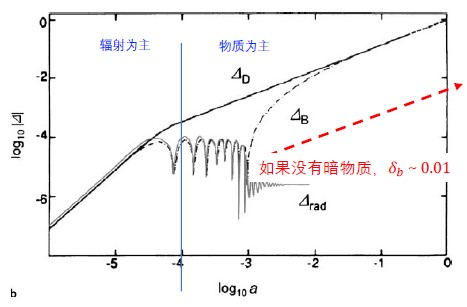
\includegraphics[width=0.42\textwidth]{GA8/扰动尺度上不同物质分量的扰动增长}
    \caption{扰动尺度$\sim 15Mpc/h\ (k=0.42h/Mpc)$上不同物质分量的扰动增长}
\end{figure}
\begin{enumerate}\small
    \item 进入视界前
    \begin{align*}
        \delta\sim\left\{\begin{array}{ll}
            a^2&\text{辐射主导}\\
            a &  \text{物质主导}
        \end{array} \right.
    \end{align*}
    \item 进入视界后, 辐射为主, 再复合前
    \begin{itemize}
        \item 光子: 声波震荡
        \item 重子: 声波震荡
        \item 暗物质: $\delta\sim \ln a$
    \end{itemize}
    \item 进入视界后, 物质为主,再复合前
    \begin{itemize}
        \item 光子: 声波震荡
        \item 重子: 声波震荡
        \item 暗物质: $\delta\sim a$
    \end{itemize}
    \item 复合之后
    \begin{itemize}
        \item 光子: 声波震荡
        \item 重子: $\delta\sim a$
        \item 暗物质: $\delta\sim a$
    \end{itemize}
\end{enumerate}

\begin{figure}[!htb]
    \centering
    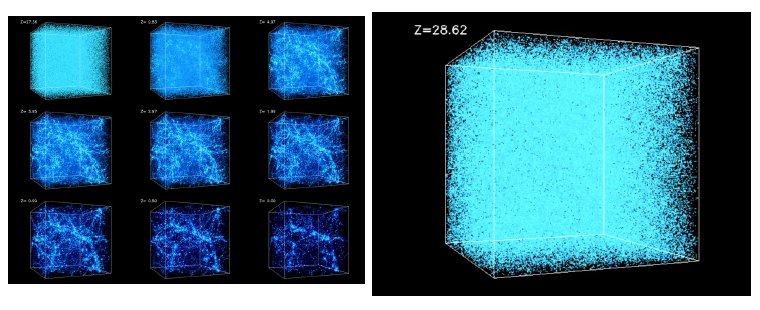
\includegraphics[width=0.42\textwidth]{GA8/大尺度上, 物质形成宇宙网络结构}
    \caption{大尺度上, 物质形成宇宙网络结构}
\end{figure}

\subsection{球塌缩模型}
当某些区域密度扰动变得接近于 $\delta\sim 1$时, 线性扰动理论失效, 发生物质塌缩, 形成暗物质晕(dark matter halo). 

最简单的球塌缩模型预言, 暗晕内的平均密度$\sim 200\rho$($\rho$为宇宙背景的平均密度)
\begin{align*}
    \rho=\Omega_m\rho_c=\Omega_m\frac{3H^2}{8\pi G}
\end{align*}

从数值模拟中寻找暗晕: 以某处密度最高点为中心, 寻找某一个半径, 其内的物质平均密度为宇宙背景密度的$\sim 200$倍 (具体数值依赖于宇宙学参数, 但是变化不大)可得到暗晕的位力质量$M_{vir}$, 和半径$R_{vir}$. 

\begin{figure}[!htb]
    \centering
    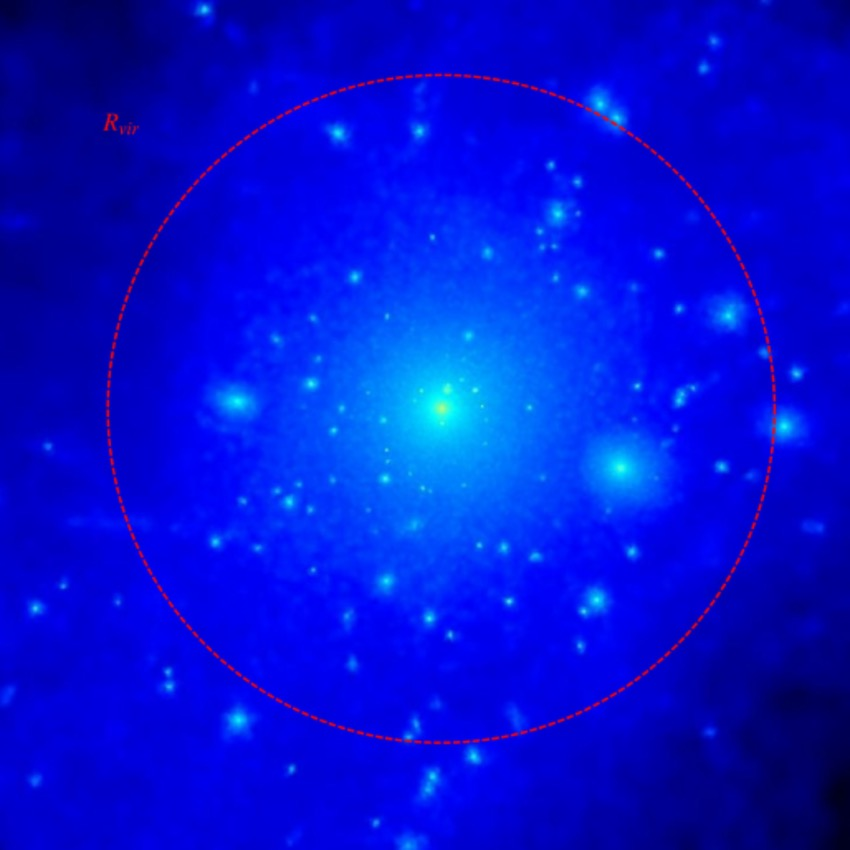
\includegraphics[width=0.309\textwidth]{GA8/球塌缩模型}
    \caption{球塌缩模型}
\end{figure}


\subsubsection{暗晕密度分布(Halo density profile)}

\begin{figure}[!htb]
    \centering
    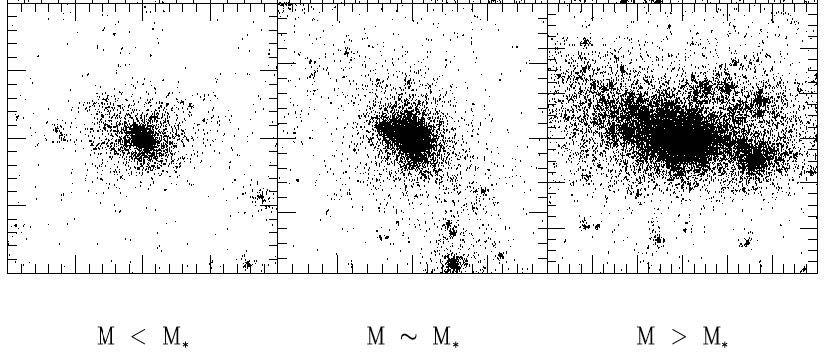
\includegraphics[width=0.42\textwidth]{GA8/数值模拟中暗晕的形状}
    \caption{数值模拟中暗晕的形状}
\end{figure}

\begin{figure}[!htb]
    \centering
    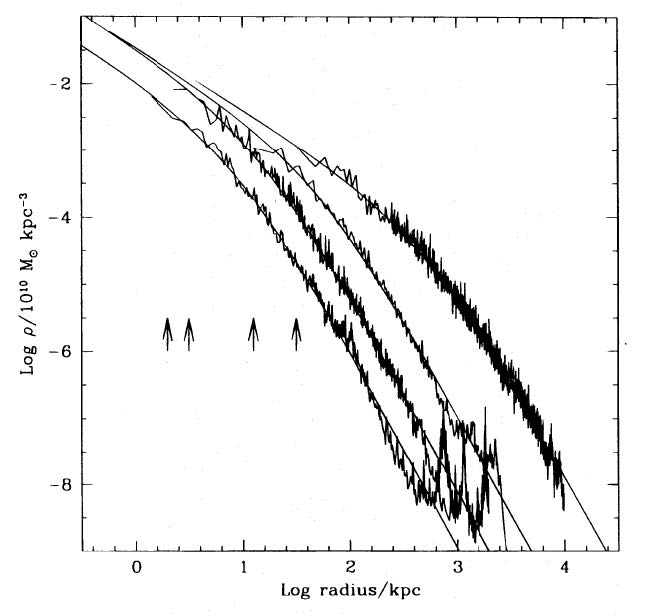
\includegraphics[width=0.309\textwidth]{GA8/不同质量暗晕的密度轮廓}
    \caption{不同质量暗晕的密度轮廓$\rho(r)$, $r$为距离暗晕中心的距离. $\rho$随$r$减小而增加, 给定$r$, 暗晕质量越大, $\rho$越高}
\end{figure}

尽管每个暗晕的密度各不相同, 但是Navarro, Frenk, White等人(1996,1997)发现, 暗晕密度轮廓具有相似的形式, 提出了著名的NFW Profile
\begin{align}
    \rho(r)=\frac{\rho_{crit}\delta_c}{\frac{r}{r_s}\left( 1+\frac{r}{r_s} \right)^2}\label{EE12}
\end{align}
这里$\rho_{crit}=\frac{3H^2}{8\pi G}$, 是宇宙某一时刻的临界密度, 只与时间有关, 与暗晕质量无关. $r_s=\frac{R_{vir}}{c}$是暗晕的特征半径, $R_{vir}$是暗晕的位力半径, $c$为聚集度(Concentration). 该表达式几乎不依赖于宇宙学模型和宇宙时间. 因此被广泛用于计算暗晕的质量分布和旋转曲线. 

球塌缩模型预言暗晕质量和半径满足
\begin{align*}
    M_{vir}=\frac{4\pi}{3}200\rho_c R_{vir}^3
\end{align*}
因此只要给定$M_{vir}$, 就可以得到$R_{vir}$. 积分 \ref{EE12} 到$R_{vir}$, 可得
\begin{align*}
    \delta_c=\frac{200}{3}\frac{c^3}{\left[ \ln(1+c)-\frac{c}{1+c} \right]}
\end{align*}
因此, 给定$M_{vir}$, NFW Profile 中只有一个自由参数$c$. 

{\small
研究发现, 尽管对于给定质量的暗晕, 其聚集度$c$有较大变化, 且依赖于暗晕的形成历史. 有相当多的工作发现总体来说, $c$与$M_{vir}$存在较好的相关关系, $M_{vir}$越大, $c$越小(Bullock et al. 2001; Wechsler et al. 2002; Zhao D.H. et al. 2009). 因此, 对于大部分研究, 只要确定$M_{vir}$, 就可以唯一确定暗晕的密度 Profile, 以及旋转曲线等, 这也常用来拟合观测的星系旋转曲线, 从而确定其所在$M_{vir}$. 
}

\begin{figure}[!htb]
    \centering
    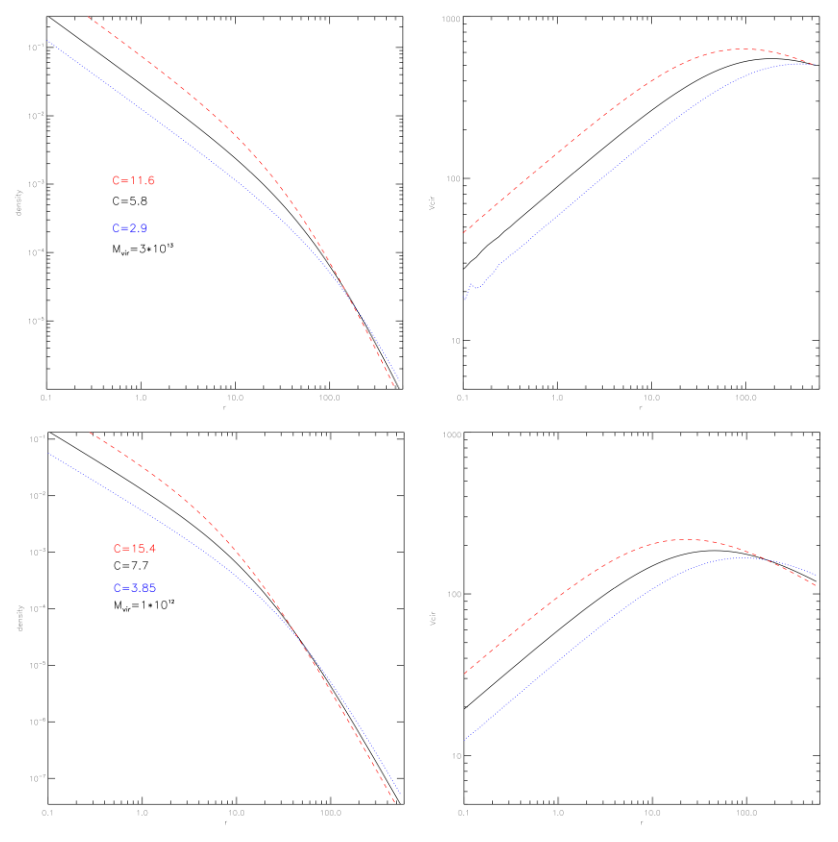
\includegraphics[width=0.42\textwidth]{GA8/2个不同质量的暗晕, 其密度, 旋转速度对C的依赖关系}
    \caption{\small 2个不同质量的暗晕, 其密度, 旋转速度对$c$的依赖关系. 给定暗晕质量, $c$越大, 内部密度和旋转速度也越大. 存在一个半径, 旋转速度达到最大值(与$c$有关)}
\end{figure}


\subsubsection{暗晕的合并和增长}
暗晕形成后并不处于静止状态, 而是在空间运动. 在暗晕运动过程中, 暗晕会相互合并(merger)并导致质量增长. 

任何暗晕都会经历合并过程. 如银河系在成长到今天的过程中, 至少经历了上千次合并(具体依赖于暗物质的性质和暗晕质量下限). 

在宇宙不同时刻, 不同尺度的结构依次形成. 在高红移, 小质量暗晕形成. 到了低红移, 暗物质晕相互并合, 形成更大质量的暗晕. 暗晕并合是宇宙中最常见的现象. 这个过程从下而上, 也称为等级成团模型. 

\begin{figure}[!htb]
    \centering
    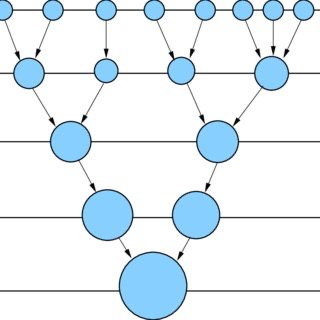
\includegraphics[width=0.309\textwidth]{GA8/暗晕的并合树 (Merger tree)}
    \caption{暗晕的并合树 (Merger tree)}
\end{figure}

\paragraph{暗晕形成历史}
暗晕的质量增长主要是通过并合和吸积弥散物质. 利用数值模拟, 人们发现, 即使对于相同质量的暗晕, 其形成历史也不一样. 一般将暗晕的形成历史形象地称为暗晕的并合树(Merger tree). 

暗晕的形成时间($z_{form}$): 暗晕历史上质量达到目前的一半. 平均来说, (今天宇宙中)质量较小的暗晕, 其形成时间也越早. 

\subsubsection{暗晕子结构}

\begin{figure}[!htb]
    \centering
    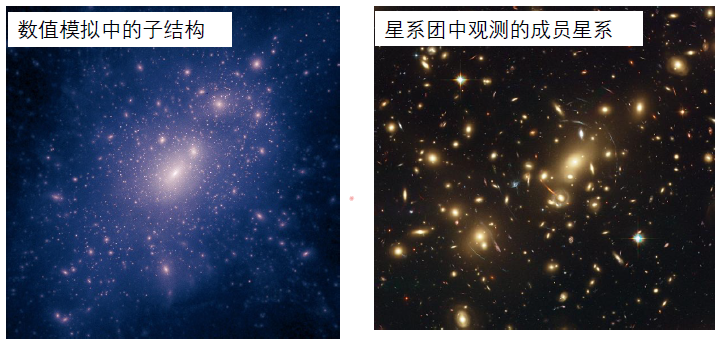
\includegraphics[width=0.42\textwidth]{GA8/暗晕子结构}
    \caption{暗晕子结构}
\end{figure}

大量低质量暗晕并合形成大质量暗晕后, 它们在大质量暗晕内并未立即消失, 而是形成子结构(Substructure, or subhalo). 这些子结构经历强烈的动力学过程
\begin{itemize}\small
    \item 潮汐剥离(tidal stripping): 大质量暗晕内部的潮汐力导致子结构质量损失. 
    \item 瓦解过程: 有些子结构经历了很强的潮汐加热, 导致其最终变成不束缚结构而解体(瓦解). 
\end{itemize}

暗晕内部的子结构是之前合并的暗晕遗迹. 每个子结构中心都可能存在恒星. 

暗晕子结构如果不存在恒星, 如何探测这些子结构?

\paragraph{数值模拟}
首先我们假设宇宙由大量的、等质量的粒子组成(粒子的具体质量$m=\frac{\bar{\rho}V}{N}$). 在初始时刻($t_i$), 宇宙的物质分布不均匀($\rho_i(x)$), 可利用泊松方程求得引力势($\psi_t(x)$), 进一步确定粒子速度($V$)和加速度(̇$\dot{V}$). 对时间积分, 确定新的粒子位置, 求得新的引力势和加速度, 得到新的位置. 一直重复到给定的时刻(如$z=0$). 

\begin{enumerate}
    \item 确定宇宙的初始条件
    \subitem 初始条件就是宇宙原初的扰动谱. 扰动谱就是在不同尺度上的扰动大小. 我们能直接观测的宇宙初始扰动来自宇宙微波背景辐射. 通过对CMB在不同尺度的温度差异, 可以确定其功率谱. 
    \begin{figure}[!htb]
        \centering
        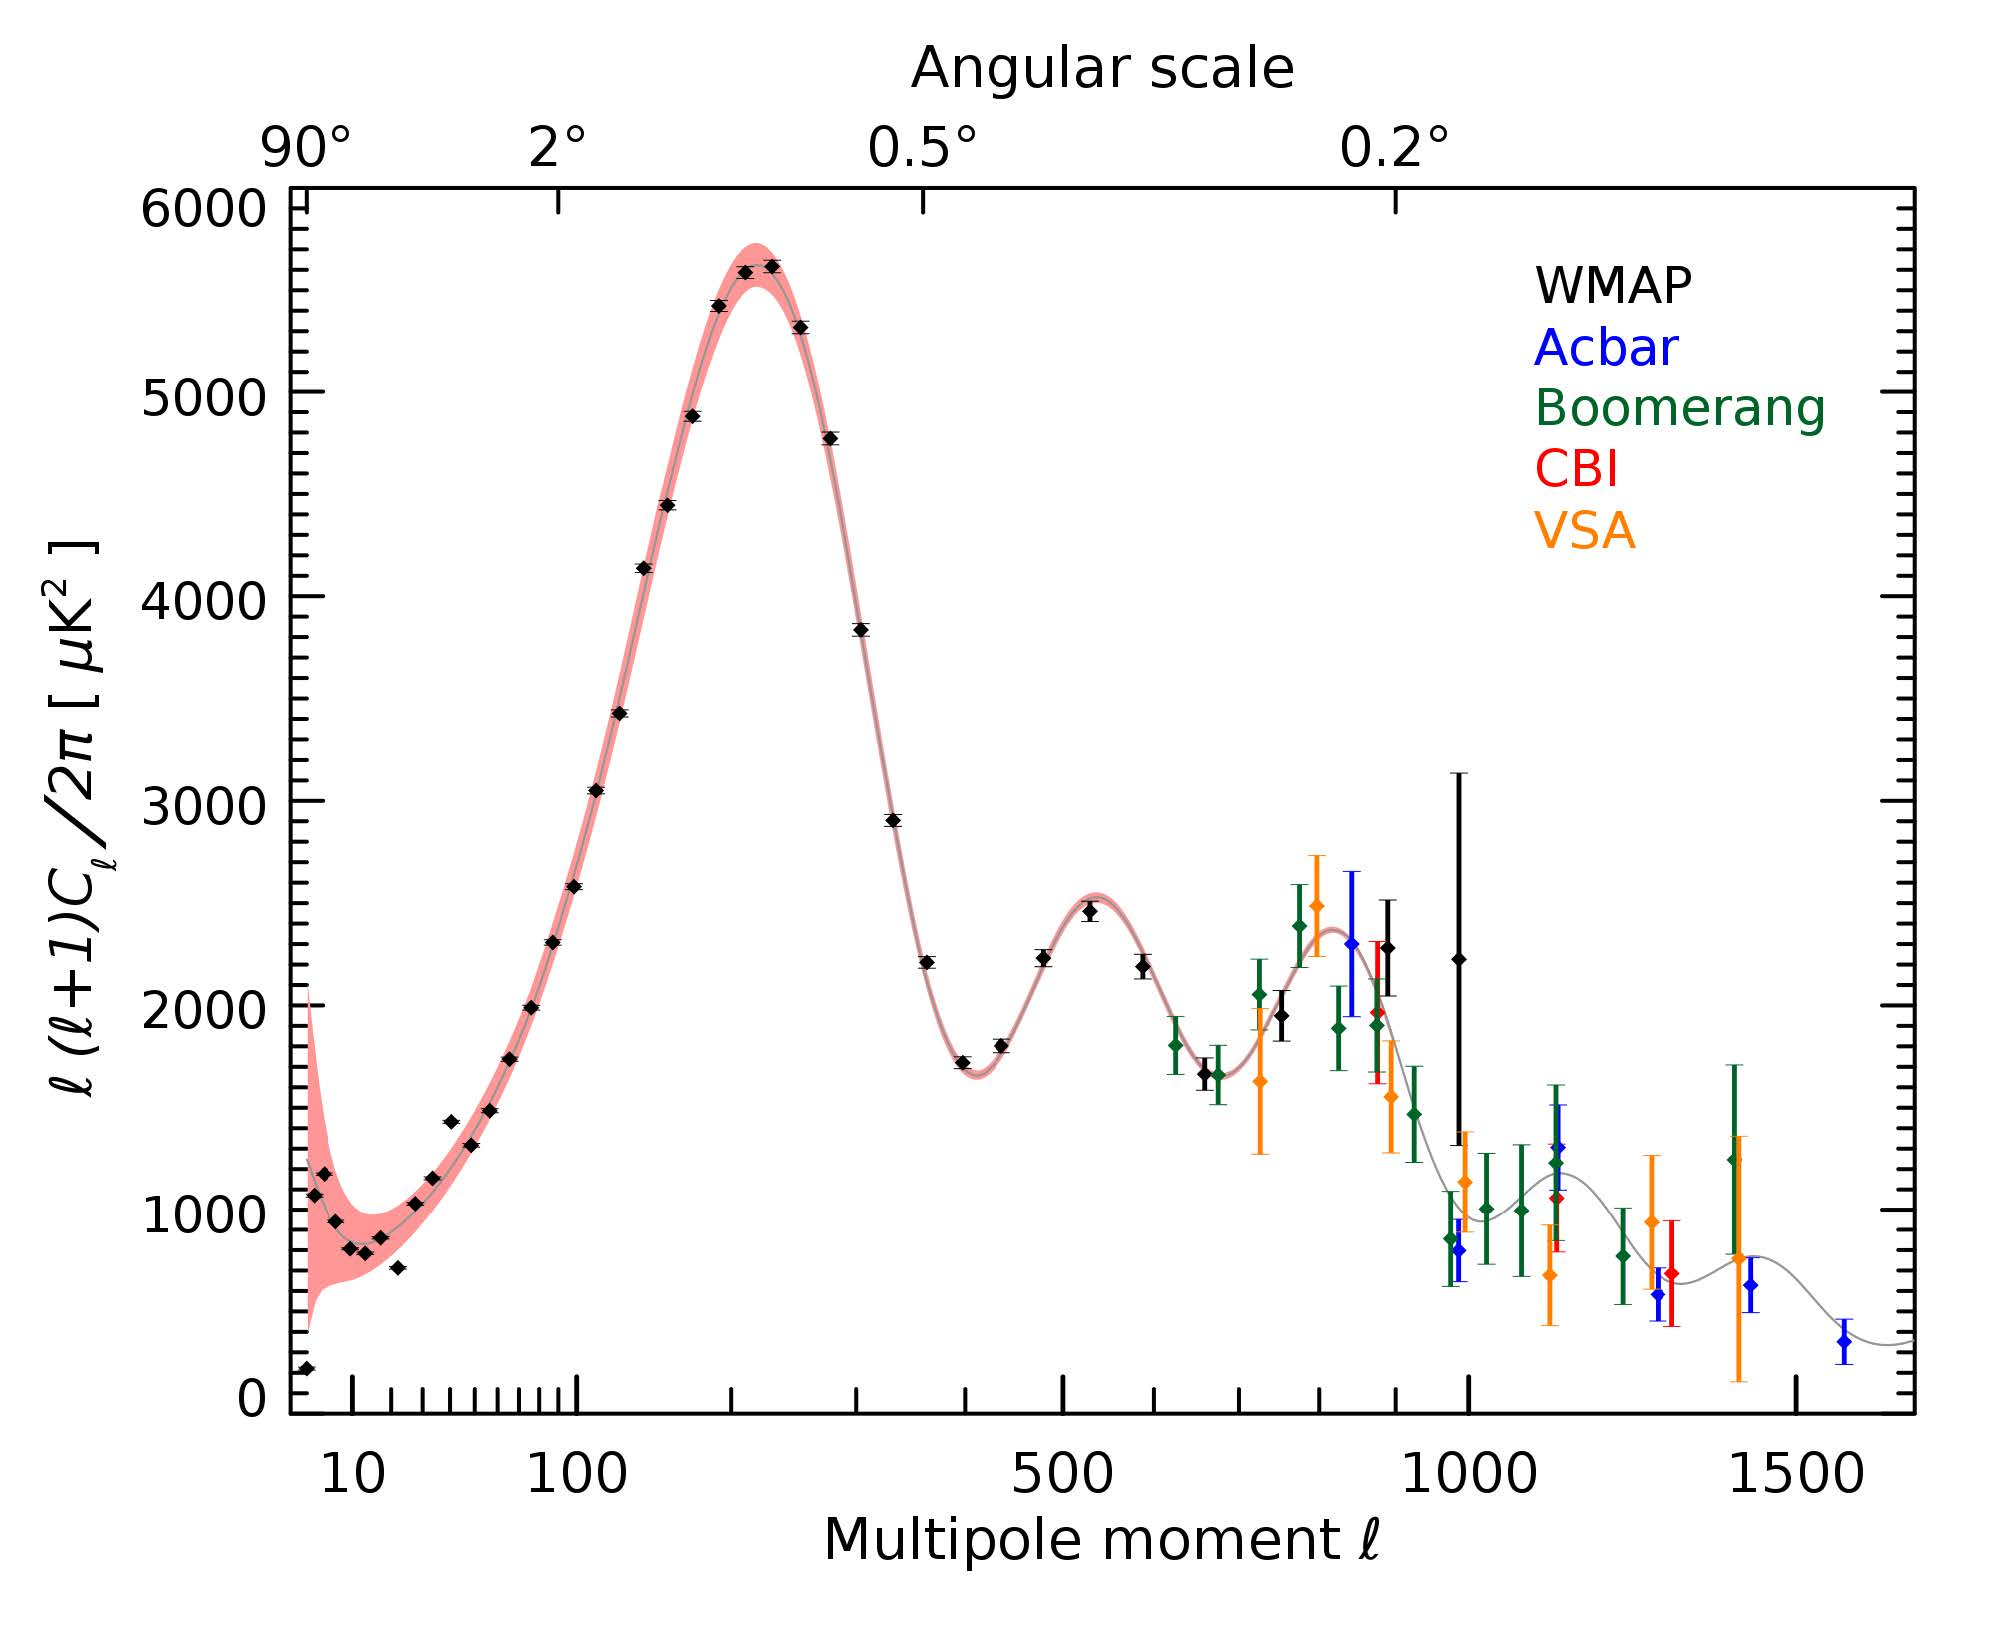
\includegraphics[width=0.42\textwidth]{GA8/对CMB Power Spectrum观测拟合}
        \caption{\small 对CMB Power Spectrum, 黑色点为WMAP卫星观测数据, 红色实线为理论预言. 通过拟合观测, 可以得到宇宙学基本参数. }
    \end{figure}
    \item 用粒子代替密度场, 并计算运动方程
    \begin{figure}[!htb]
        \centering
        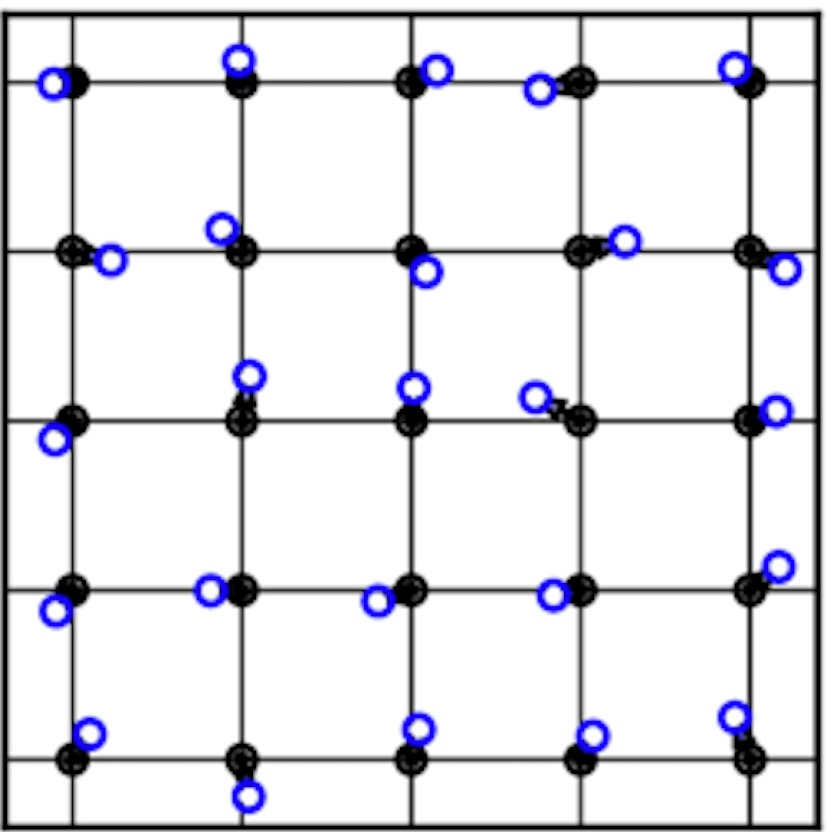
\includegraphics[width=0.22\textwidth]{GA8/空间格点}
        \caption{空间格点}
        \label{空间格点}
    \end{figure}
    \subitem 将空间分成大量等间隔的格点(如图 \ref{空间格点}, 2维情况). 根据初始时刻$t_i$的功率谱, 在每个格点位置得到其密度
    \begin{align*}
        \delta_i(x)=\sum_k\delta_i(k)e^{ikx}
    \end{align*}
    根据得到的密度$\delta_i(x)$ , 在相应位置$x$处产生对应的粒子数目(由于粒子数目不可能为整数, 实际上在最开始在每个格点放置一个粒子, 根据Zeldovich Approximation进行位置移动, 这里不详细描述, 只是原理性介绍)
    \subitem 根据(无压强)流体方程得到引力势和速度
    \begin{align*}
        \nabla^2\psi&=4\pi G\bar{\rho} a^2\delta\rho\\
        \frac{\partial v}{\partial t}+\frac{\dot{a}}{a}v&=-\frac{\nabla\psi}{a}
    \end{align*}
    根据得到的$v$, 将粒子移动到新的位置. 再次计算泊松方程, 得到新的速度, 依次循环. 
    \begin{figure}[!htb]
        \centering
        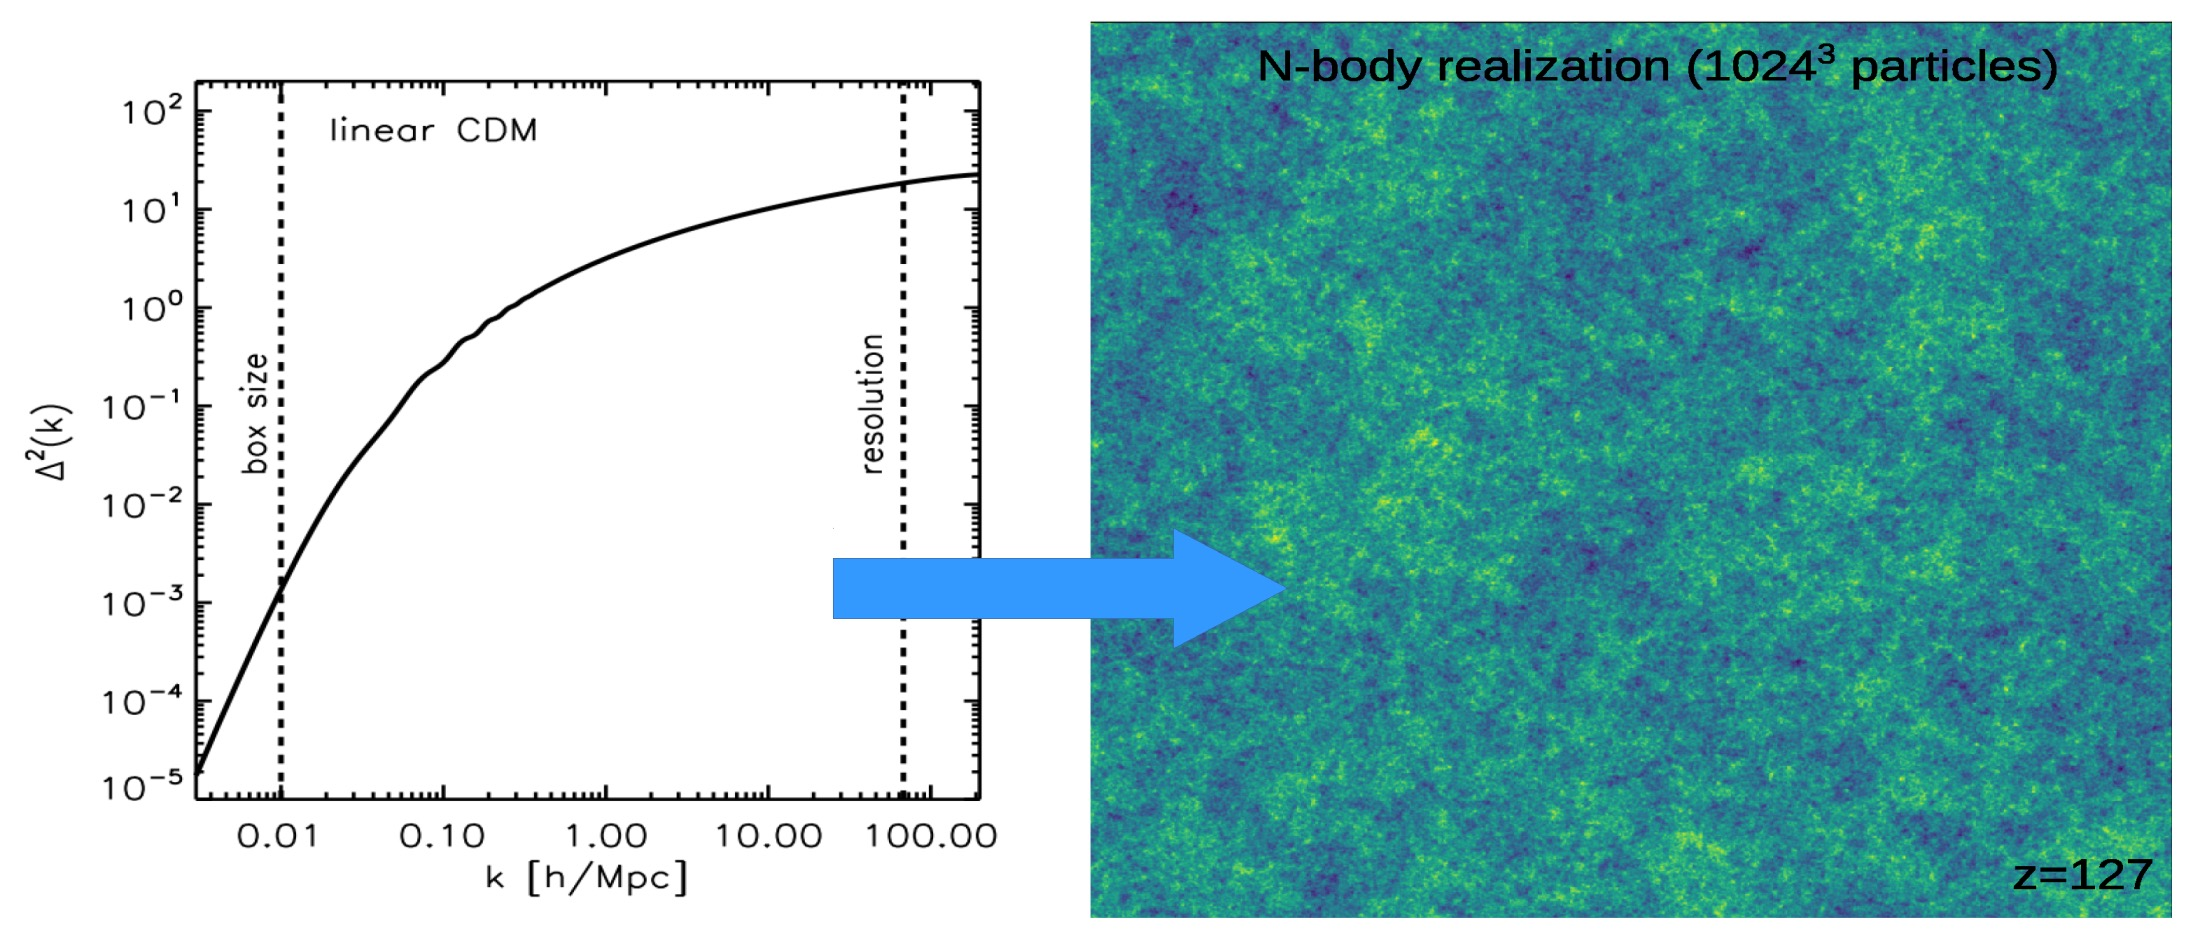
\includegraphics[width=0.42\textwidth]{GA8/用粒子代替密度场, 并计算运动方程}
        \caption{用粒子代替密度场, 并计算运动方程}
    \end{figure}
    
\end{enumerate}

\subsubsection{暗晕的质量函数(Press-Schechter Mass Function)}
在宇宙演化过程中, 任意时刻都会形成暗晕. 这些暗晕具有不同的质量. 
\begin{figure}[!htb]
    \centering
    \begin{subfigure}{0.22\textwidth}
        \centering
        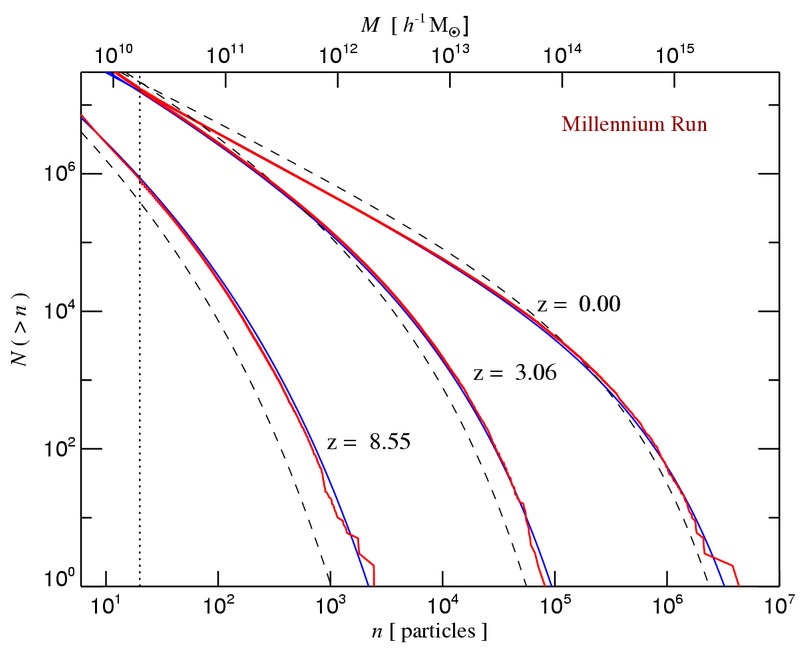
\includegraphics[width=\textwidth]{GA8/暗晕数目分布}
        \caption{暗晕数目分布}
    \end{subfigure}
    \begin{subfigure}{0.22\textwidth}
        \centering
        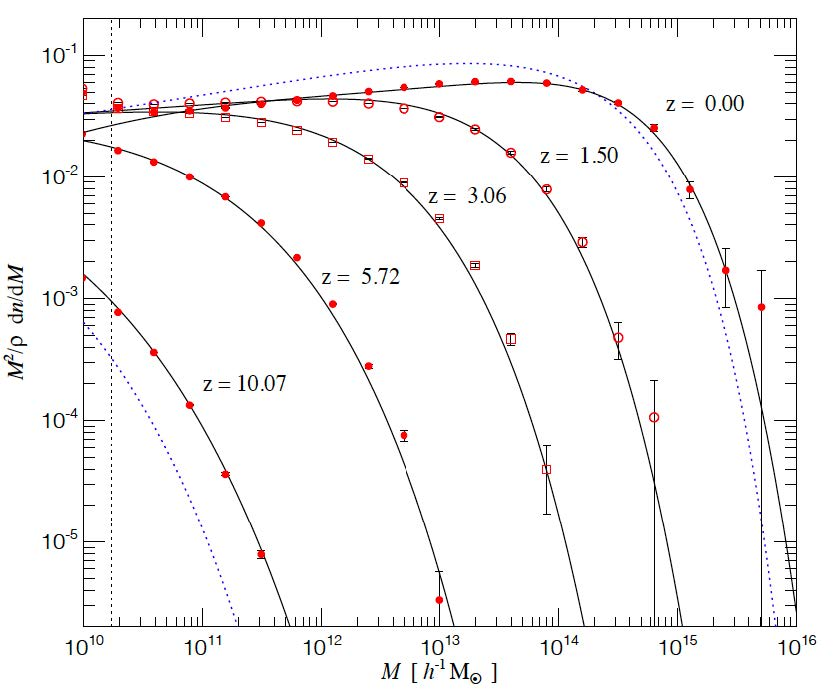
\includegraphics[width=\textwidth]{GA8/暗晕质量分布}
        \caption{暗晕质量分布}
    \end{subfigure}
    \caption{\small 数值模拟和理论预言的暗晕数目-质量分布(质量函数), 随时间的演化}
\end{figure}
\begin{itemize}\small 
    \item 暗晕的数目随质量减小而增加
    \item 暗晕数目整体随红移减小而增加(越来越多的物质进入塌缩阶段)
    \item 单位对数间隔内的总质量有演化, 到红移$z=0$时, 质量主要集中在$10^{14}$太阳质量(低质量暗晕虽然数目多, 但质量小. 大质量暗晕数目减小很快). 
\end{itemize}

\subsection{星系形成模型(Galaxy Formation Model)}
目前有三种流行的星系形成模型, 丰度匹配模型、半解析模型、包含重子的流体数值模拟. 无论那种模型, 其基本假设都是星系形成于暗晕之中, 由于暗晕内的气体冷却, 导致了恒星的形成. 
\subsubsection{丰度匹配模型(Abundance Matching Method)}
星系形成于暗晕或者暗晕子结构之中, 星系的质量与暗晕/子结构的质量(或者旋转速度)之间存在一一对应关系. 常见的做法是:
\begin{enumerate}
    \item 观测中星系按质量从大到小排序. 
    \item 将数值模拟中的暗晕子结构按质量从大到小排序. 
    \item 依次将两者进行匹配
\end{enumerate}

该方法的优点: 假设合理且简单, 其预言的星系空间分布等与观测非常一致. 

缺点: 没有涉及物理过程. 

\subsubsection{半解析模型(Semi-analytical model)}
目前广泛应用的星系形成模型之一. 

基本思想: 暗物质塌缩成暗晕, 暗晕中气体冷却, 恒星形成. 暗晕的相互并合导致星系的并合, 形成了形态各异的星系. 由于其结合了暗晕形成的强烈非线性过程(只能利用数值模拟给出完整描述)和星系形成的物理解析过程, 因此被称
为半解析模型. 

\begin{figure}[!htb]
    \centering
    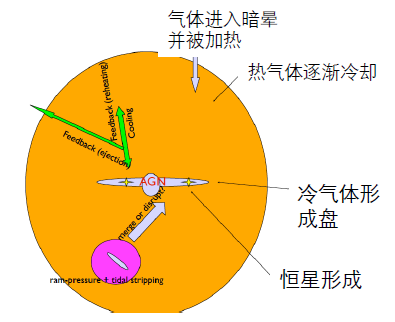
\includegraphics[width=0.309\textwidth]{GA8/半解析模型}
    \caption{半解析模型}
\end{figure}

\paragraph{热气体冷却并形成冷气体盘}
\begin{figure}[!htb]
    \centering
    \begin{tikzpicture}
        \draw (0, 0) [fill=red, draw=black] circle (2);
        \draw (0, 0) [fill=light_blue, draw=black] circle (1.2);
        \draw [->, white] (0,0)--(30:1.2) node [midway, above] {$r_{cool}$};
    \end{tikzpicture}
\end{figure}

假设气体为等温球分布
\begin{enumerate}
    \item 暗晕内气体被加热到暗晕的位力温度
    \begin{align*}
        T=\frac{1}{2}\frac{um_p}{k}V_{vir}^2
    \end{align*}
    \item 由于气体温度高, 原子被电离, 产生韧制辐射, 其单位时间的辐射能量为
    \begin{align*}
        E=n_e^2(r)\Lambda(T, Z)
    \end{align*}
    $\Lambda$为冷却函数, 依赖于气体的金属丰度和温度, 因此半径$r$处气体冷却时间为
    \begin{align*}
        t_{cool}(r)=\frac{3}{2}\frac{kT\rho(r)}{um_p}\frac{1}{E}
    \end{align*}
    \item 给定暗晕的年龄$t_{age}$, 计算冷却半径$r_{cool}$, 使得$t_{age}=t_{cool}(r_{cool})$
    \item 冷却半径$r_{cool}$内的气体形成冷气体盘, 其大小通常为暗晕位力半径的$10\%$
\end{enumerate}

\paragraph{恒星形成率--Kennicutt-Schmidt law}
对于冷气体, 由于引力不稳定性, 一旦扰动尺度超过金斯质量, 气体将塌缩并形成恒星. Schmidt (1959),  Kennicutt (1998)总结了大量观测数据, 发现星系中恒星形成率与气体总面密度之间存在很好的相关关系. 这一关系也被称为Kennicutt-Schmidt Law, 广泛应用于星系形成模型之中. 

KS Law可以表示为
\begin{align*}
    \dot{\Sigma}_*=(2.5\pm 0.7)\times10^{-4}\left( \frac{\Sigma_{gas}}{M_{\odot}pc^{-2}} \right)^{1.4\pm 0.15}M_{\odot}yr^{-1}kpc^{-2}
\end{align*}
$\Sigma_*$表示恒星形成的面密度. 

半解析模型中, 通常假设
\begin{align*}
    \dot{M}_*=\alpha\frac{M_{cold}}{\tau_{dyn}}
\end{align*}
实际上, 恒星形成于分子云, 因此应该只与分子气体面密度有关. 但是上述关系仍然非常精确. 

\paragraph{超新星反馈}
大质量恒星演化到晚期会发生超新星爆炸. 其释放出大量能量和物质到周围的冷气体中, 引起大量气体物质外流, 其外流速度可达1000km/s. 目前普遍认为超新星反馈对星系形成有着非常关键的作用. 

大质量恒星的比例: 依赖于IMF. 对于Salpeter形式的恒星初始质量函数, 大质量恒星的质量占比$\eta_{SN} \sim 6.3\times10^{-3}$. 每个超新星爆发的能量$E_{SN}\sim 10^{51}$erg. 因此, 单位超新星爆炸释放的总能量
\begin{align*}
    \Delta E=\epsilon E_{SN}\dot{M}_*
\end{align*}
一般假设其中有𝜖比例的能量用来加热周围的冷气体, 将其加热到暗晕的位力温度, 并形成外流, 因此被加热气体的总量
\begin{align*}
    \Delta M_{heat}=\frac{4}{3}\frac{\epsilon \Delta E}{V_{vir}^2}
\end{align*}

外流气体的命运: 非常不确定, 早期模型认为其停留在暗晕内, 与其热气体混合. 也有模型认为其逃离暗晕, 直到被再次吸积. 

需要利用数值模拟从第一性原理出发, 详细研究
\begin{itemize}
    \item  超新星爆炸有多少比例$\epsilon$的能量进入周边冷气体
    \item 外流气体是如何在星系环境下进行循环的
\end{itemize}


\paragraph{星系合并及星暴}
暗晕之间频繁发生并合, 其中的星系经历动力学摩擦也随之并合. 
\begin{figure}[!htb]
    \centering
    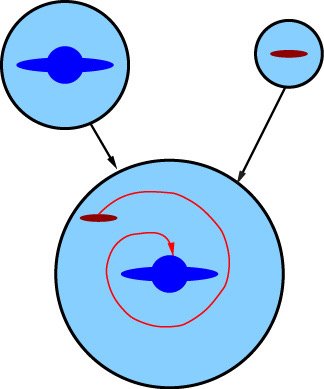
\includegraphics[width=0.12\textwidth]{GA8/星系合并}
    \caption{星系合并}
\end{figure}

数值模拟发现, 动力学摩擦时标可以近似为
\begin{align*}
    T_{df}=\frac{1}{2}\frac{f(\epsilon)}{0.43}\frac{V_{vir}R_{vir}^2}{GM_{sat}\ln \Lambda}
\end{align*}
并合时间一般从$0.5 Gyr\sim 10 Gyr$. 低质量星系甚至在哈勃时标内都不并合(如星系团中的成员星系). 

并合时, 强烈的潮汐作用导致大量的恒星形成(星爆 star burst). 根据并合时星系的质量之比, 一般将并合分为主并合(Major Merger, $>1/3$)和次并合(Minor merger, $<1/3$). 
\begin{itemize}
    \item 在Minor Merger中, 只有部分(具体比例非常复杂)气体在极短时间内转化为恒星. 
    \item 在Major Merger中, 几乎所有的气体全部形成恒星, 形成星暴星系. 并合结束后, 所有的恒星形成一个核球, 形成椭圆星系. 
\end{itemize}

\paragraph{黑洞的形成及反馈}
研究发现几乎所有的星系中心都有一个大质量黑洞, 其质量与星系核球质量有非常好的相关关系$M_{bh}\sim 0.002M_{bulge}$ (Magorrian et al. 1998, 有时也称为Magorrial relation, Mbh-Mbulge relation).

Kauffmann等(2000)认为黑洞主要在星系并合时发生增长, 并引入黑洞的质量增加为:
\begin{align*}
    M_{bh, acc}=\frac{f_{BH}M_{cold}}{1+\left( \frac{280}{V_{vir}} \right)^2}
\end{align*}
黑洞吸积产生能量, 大约0.05的能量($0.05M_{bh,acc}c^2$)释放到星系周边, 并用来加热暗晕内的热气体, 抑制其冷却. 

上述模型非常简单, 以至于很难描述实际情况. 目前所有模型, 流体模拟的重点就是模拟黑洞的吸积及反馈过程. 困难在于两者尺度相差实在太大$(10^{12})$, 无法同时解析这样大范围的尺度. 

\paragraph{星族合成及其他}
上述过程只描述了恒星的形成过程, 但是与实际观测相比, 我们需要预言星系的能谱, 在不同波段的光谱. 这可以利用BC03等星族合成模型. 

\paragraph{尘埃的吸收和在发射}
尘埃会吸收大质量恒星在紫外的辐射, 造成星系在紫外和光学波段的吸收(遮挡), 同时, 尘埃会将吸收的能量在远红外, 亚毫米等波段辐射出来. 

\begin{figure}[!htb]
    \centering
    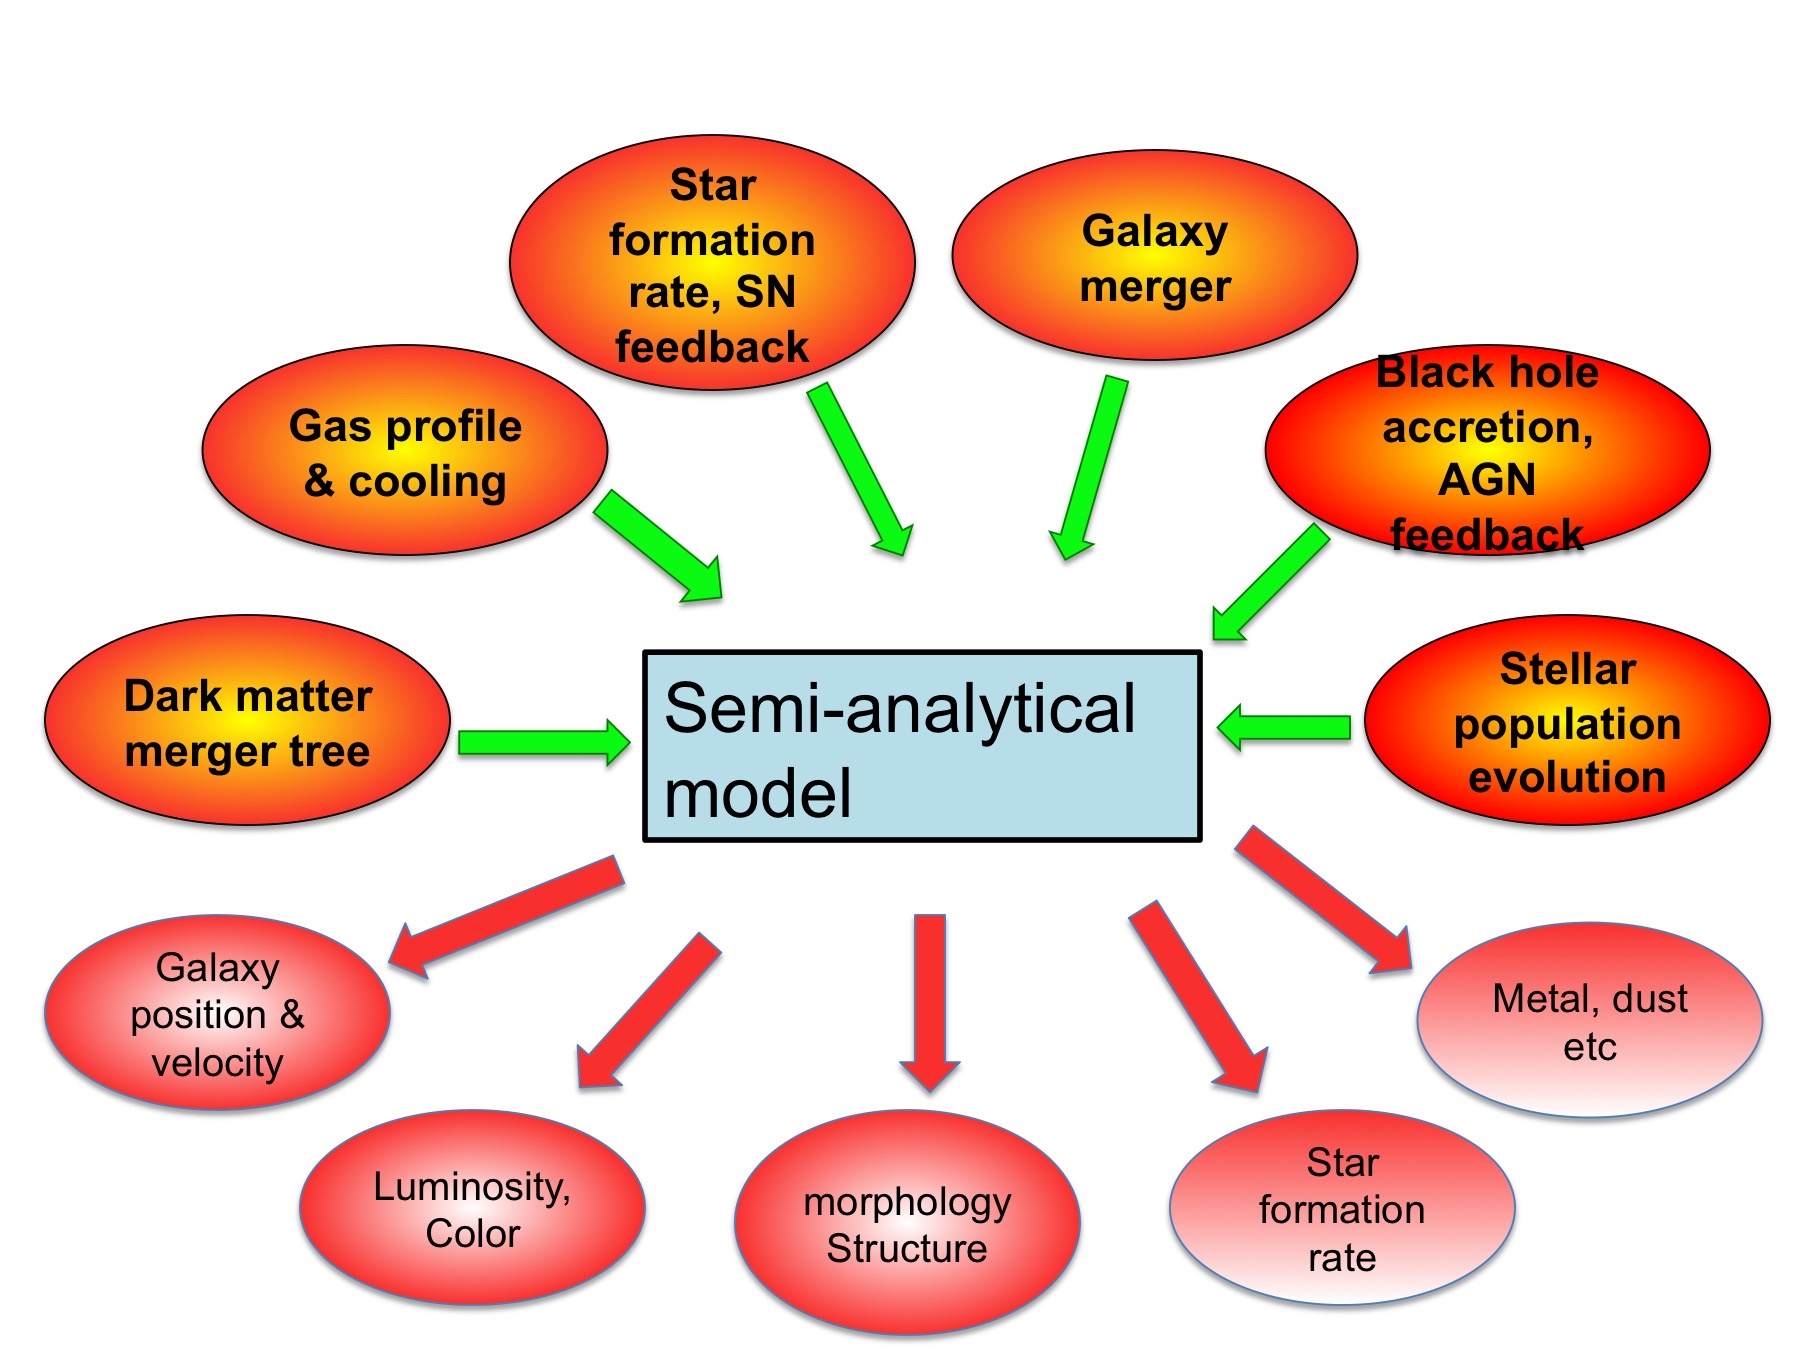
\includegraphics[width=0.42\textwidth]{GA8/半解析模型考虑以上所有物理过程}
    \caption{半解析模型考虑以上所有物理过程}
\end{figure}


\subsubsection{流体数值模拟(Hydro-dynamical simulation)}
如今, 流体模拟是研究星系形成的重要手段. 其同时模拟暗物质在宇宙中的演化, 结合几乎所有的物理过程(气体冷却, 吸积, 恒星形成, 黑洞吸积, 超新星和黑洞反馈等物理过程), 从而预言星系的形成. 

\begin{figure}[!htb]
    \centering
    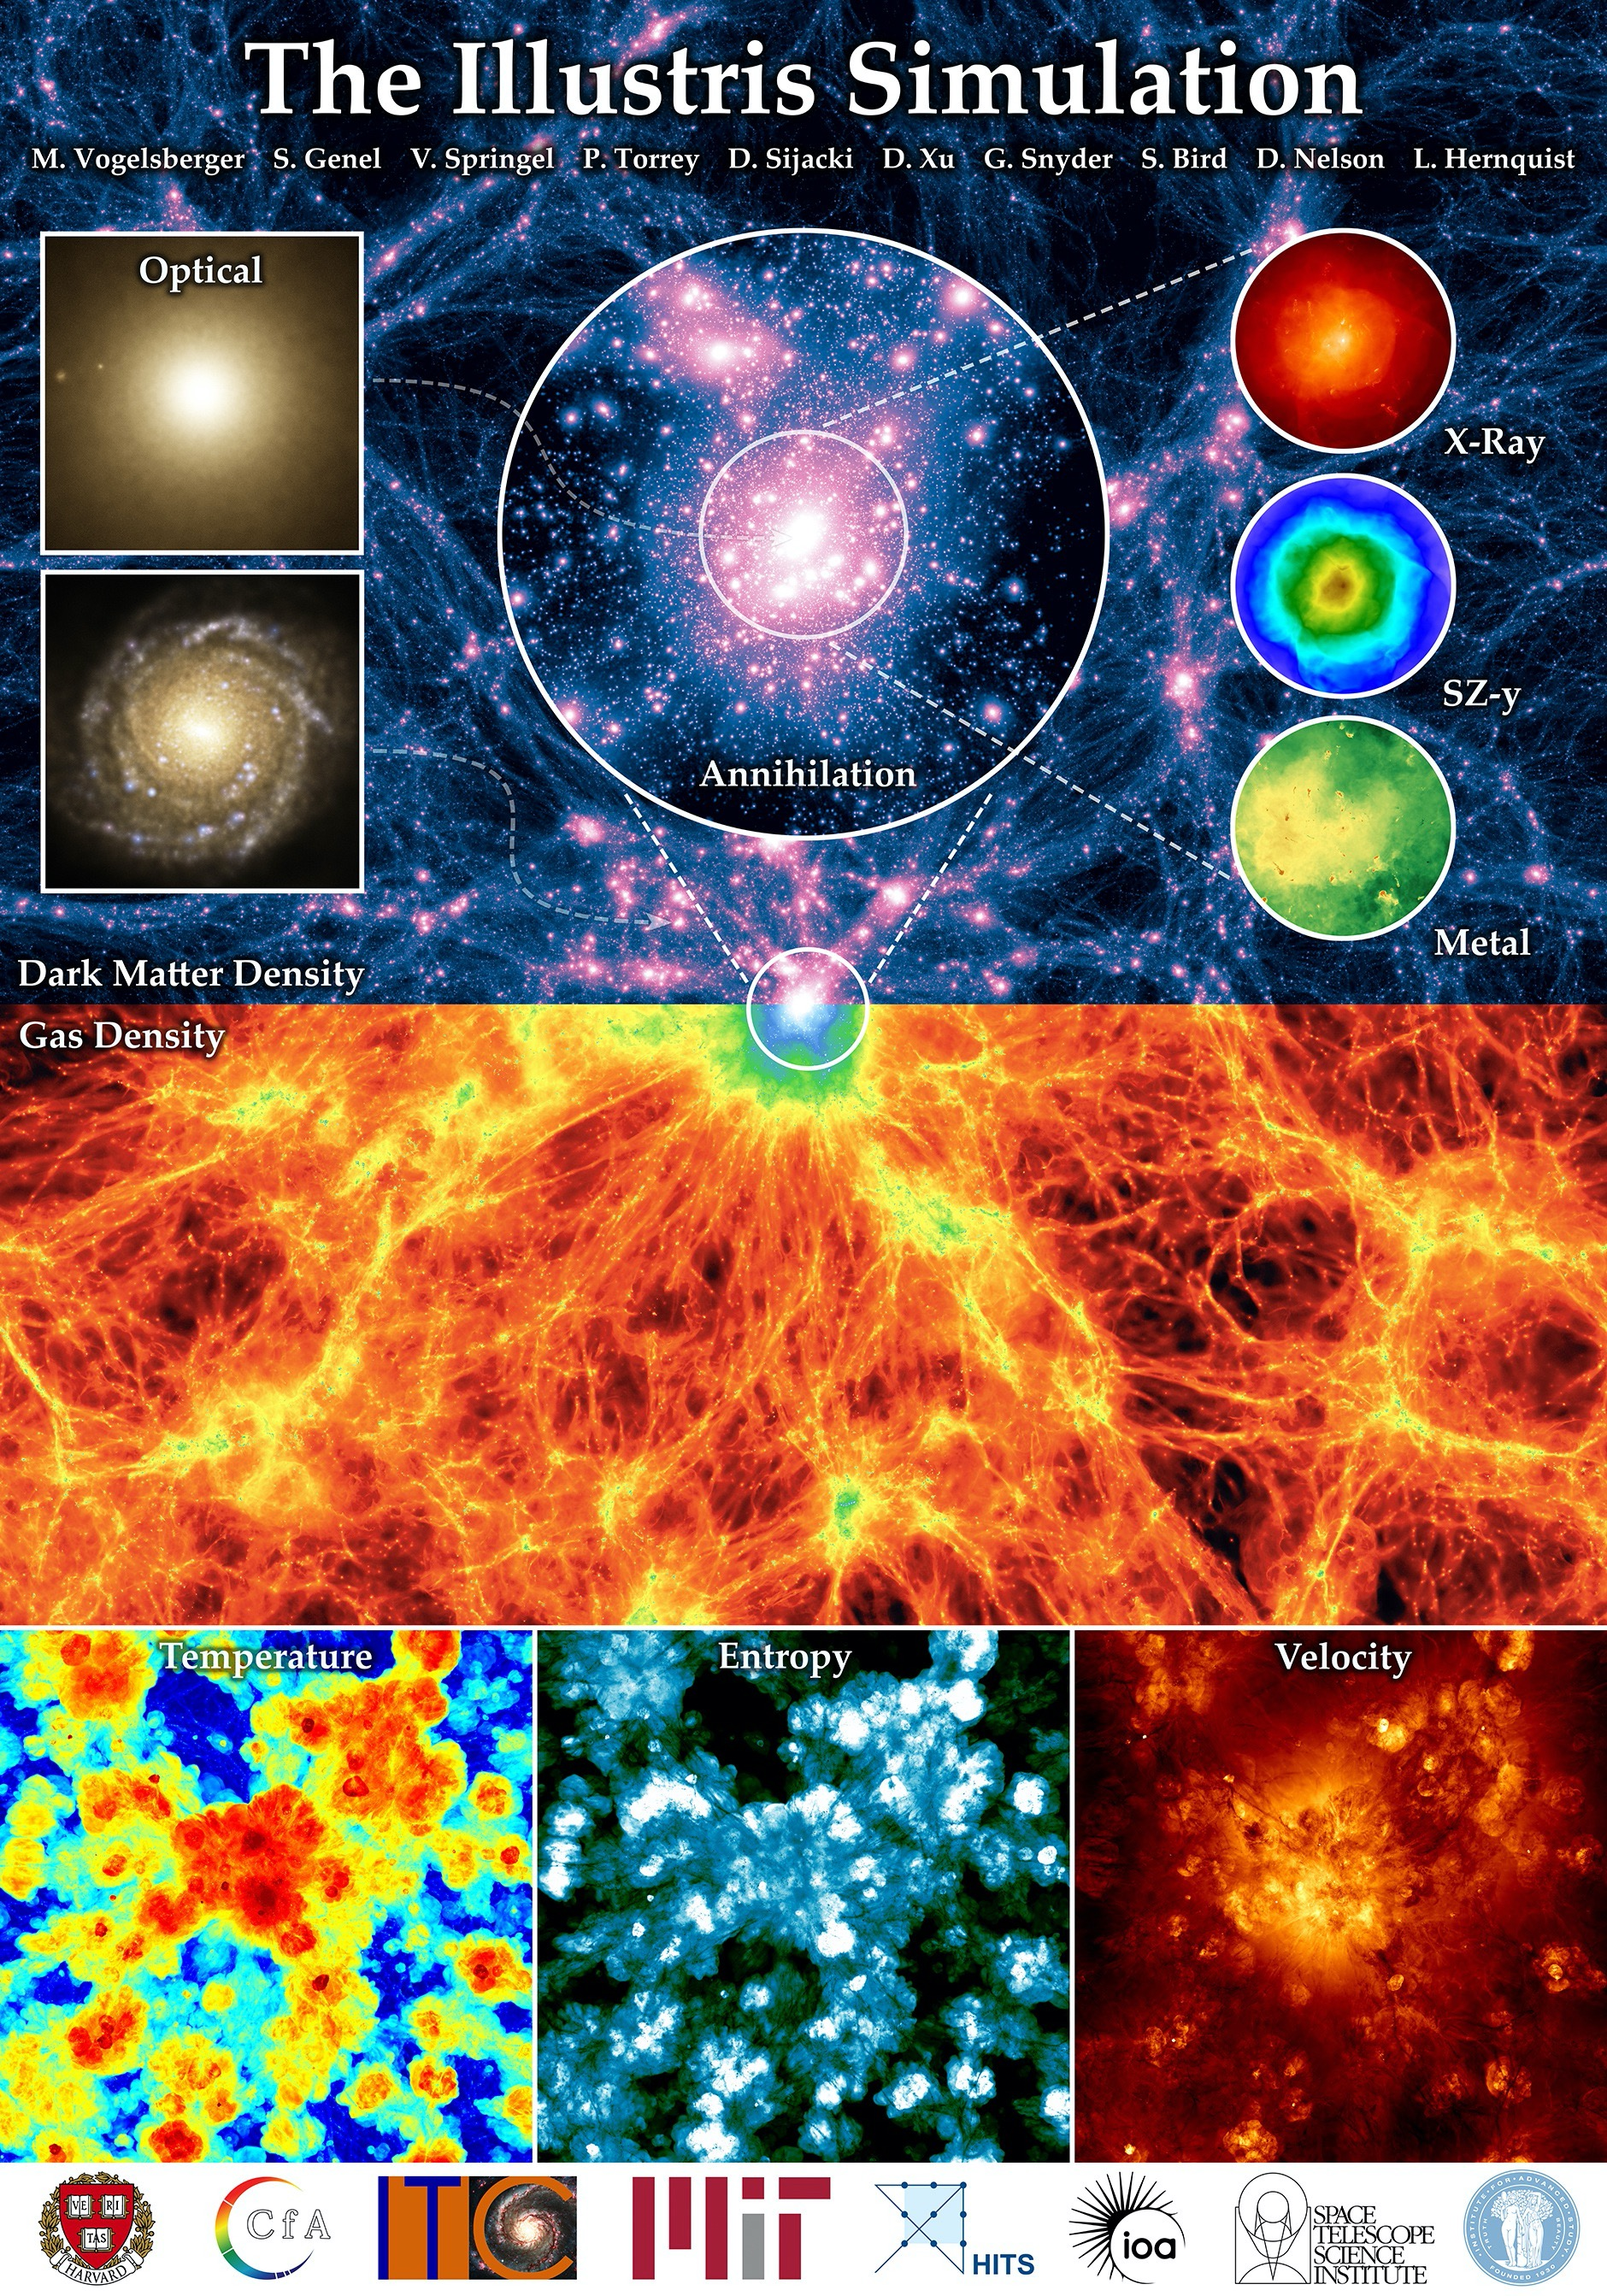
\includegraphics[width=0.309\textwidth]{GA8/流体数值模拟}
    \caption{流体数值模拟}
\end{figure}


% \section{大尺度结构统计分析}